%!TEX program = xelatex
% !Mode:: "TeX:UTF-8"
%% 请使用 XeLaTeX 编译本文.
% \documentclass{WHUBachelor}% 选项 forprint: 交付打印时添加, 避免彩色链接字迹打印偏淡. 即使用下一行:
 \documentclass[forprint]{WHUBachelor}

\begin{document}
%%%%%%% 下面的内容, 据实填空.

\miji{ }                                      % 密级. 没有就空着.
\StudentNumber{2017301500335} % 填写自己的学号

\title{基于多层感知机网络的手写数字数据集分类算法及其优化}
\Etitle{An Optimized Classifying Algorithm Based on Multi Layer Perceptron} % 英文题目
\author{张永康}                            % 作者名字
\Eauthor{Zhang Yongkang}            %作者英文名
\Csupervisor{谭成予\quad 副教授}        %指导教师中文名、职称
\Esupervisor{Prof.~TAN Chengyu}     %指导教师英文名、职称
\Cmajor{计算机类}                  % 专业中文名
\Emajor{Computing Science}% 专业英文名
\Cschoolname{计算机学院}          % 学院名
\Eschoolname{School of Computer} %学院英文名. 不确定的话, 请看一下自己学院的网页上是怎么写的. 别搞错了!
\date{二〇一八年五月}                    % 日期, 要注意和英文日期一致!!
\Edate{May, 2018}                       % 英文封面日期

%-----------------------------------------------------------------------------
\pdfbookmark[0]{封面}{title}         % 封面页加到 pdf 书签
\maketitle
\frontmatter
\pagenumbering{Roman}              % 正文之前的页码用大写罗马字母编号.
%-----------------------------------------------------------------------------
% !Mode:: "TeX:UTF-8"

%%% 此部分需要自行填写: (1) 中文摘要及关键词 (2) 英文摘要及关键词
%%%%%%%%%%%%%%%%%%%%%%%%%%%%%

%%% 郑重声明部分无需改动

%%%---- 郑重声明 (无需改动)------------------------------------%
%\newpage
%\vspace*{20pt}
%\begin{center}{\ziju{0.8}\textbf{\songti\zihao{2} 郑重声明}}\end{center}
%\par\vspace*{30pt}
%\renewcommand{\baselinestretch}{2}

%{\zihao{4}%

%本人呈交的学位论文, 是在导师的指导下, 独立进行研究工作所取得的成果,
%所有数据、图片资料真实可靠. 尽我所知, 除文中已经注明引用的内容外,
%本学位论文的研究成果不包含他人享有著作权的内容.
%对本论文所涉及的研究工作做出贡献的其他个人和集体,
%均已在文中以明确的方式标明. 本学位论文的知识产权归属于培养单位.\\[2cm]

%\hspace*{1cm}本人签名: $\underline{\hspace{3.5cm}}$
%\hspace{2cm}日期: $\underline{\hspace{3.5cm}}$\hfill\par}
%------------------------------------------------------------------------------
\baselineskip=23pt  % 正文行距为 23 磅
%------------------------------------------------------------------------------





%%======中文摘要===========================%
\begin{cnabstract}
  手写数字分类问题是机器学习与模式识别领域的基础问题之一,
  也是OCR(光学字符识别)的核心技术,具有重要的现实意义。
  本文针对MNIST手写数字数据集,通过C++实现了基于多层感知机网络
  的手写数字数据集分类算法,并采用交叉验证、小批量随机梯度
  下降算法、扩充训练数据集的方法优化算法,
  最终达到了98.042\%的分类准确率。


\end{cnabstract}
\par
\vspace*{2em}


%%%%--  关键词 -----------------------------------------%%%%%%%%
%%%%-- 注意: 每个关键词之间用“;”分开,最后一个关键词不打标点符号
\cnkeywords{多层感知机; 手写数字; 分类; 优化; }


%%====英文摘要==========================%


\begin{enabstract}
  The classification of handwritten digits is one of the basic problems of machine learning and pattern recognition, 
  which is also the key technology of optical character recognition(OCR). 
  In this paper, according to the MNIST handwritten digits dataset, 
  we implement a classifying algorithm based on multi-layer perceptron(MLP) by C++, 
  and optimize it by cross-validation, mini-batch stochastic gradient descent algorithm 
  and expanding the training dataset. 
  The accuracy of our algorithm reaches 98.042\%.

\end{enabstract}
\par
\vspace*{2em}

%%%%%-- Key words --------------------------------------%%%%%%%
%%%%-- 注意: 每个关键词之间用“;”分开,最后一个关键词不打标点符号
 \enkeywords{Multi-layer Perceptron; Handwritten Digits; Classification; Optimization;}
    % 加入摘要, 申明.
%==========================把目录加入到书签==============================%%%%%%
\pdfbookmark[0]{目录}{toc}
\tableofcontents
\mainmatter %% 以下是正文
%%%%%%%%%%%%%%%%%%%%%%%%%%%--------main matter-------%%%%%%%%%%%%%%%%%%%%%%%%%%%%%%%%%%%%
\chapter{MNIST手写数字数据集}
 
  MNIST(Mixed National Institute of Standards and Technology database)是一个包含70000个
  28×28像素大小的手写阿拉伯数字灰度图片的大型数据集\upcite{mnistdb}。MNIST数据库被广泛用于测试机器学习算法的分类能力。
  
  本文使用Kaggle在线大数据测试平台的MNIST测试系统\upcite{kaggle}来检验分类算法的分类正确率,该系统将MNIST数据库中的42000个数字作为训练集,28000个数字作为测试集。其中,每个图片被转换为28×28=784维的向量。训练集为42000行、785列的矩阵,矩阵中第i行第1列代表第i张图片对应的数字,之后的784列分别代表第i张图片中每个像素点的灰度值。测试集训练集为28000行、784列的矩阵,矩阵中第i行第j列代表第i张图片中像素点j的灰度值。

\chapter{MNIST数据集的分类算法比较}

  MNIST数据集的分类算法有很多,如K近邻算法、支持向量机\upcite{svm}、集成学习方法、多层感知机网络、
  卷积神经网络等。目前分类准确率最高的是基于胶囊网络(Capsule Network)的分类算法\upcite{capsule},
  其准确率为99.75\%。

  K近邻算法(K Nearest Neighbors,KNN)是一种度量学习方法,它基于某种距离度量,在训练
  集中找到与测试对象最近的K个训练数据,并在这K个数据中选取出现频率最高的数据类别作为测试对象
  的所属类别,具有算法容易实现的特点。但其无训练过程,在对每个数据对象进行分类时需要遍历整个
  数据集,耗时过长。

  支持向量机(Support Vector Machine,SVM)将数据映射到高维空间,使用
  核函数(Kernel Function)寻找合适的超平面划分数据集,
  与线性回归算法相比,SVM可以划分原始空间中线性不可分的数据集,具有
  计算量小、不易过拟合等优点,但数学推导过程过于复杂。

  集成学习方法(如Adaboost、随机森林)是通过构建并结合多个分类器来完成训练、分类任务。集成学习通过一定的策略训练每个子分类器、结合每个子分类器的分类结果,常常能获得比单个子分类器更好的分类准确率,具有泛化能力强的优点,缺点是算法难以理解、实现。

  多层感知机网络(Multi Layer Perceptron,MLP)是由若干层感知机神经元组成的全连接网络。其中每个神经元可以解决一个线性可分问题。MLP通过多层神经元的共同作用,可以解决大多数的线性不可分问题,其结构简单,算法易于实现,缺点是训练速度略慢,无法提取图片中的空间关系,有时需要通过特征工程对输入数据进行特征提取。

  卷积神经网络(Convolutional Neural Network,CNN)是由若干卷积层、下采样层组成的神经网络,通过卷积层的卷积核提取图片中的特征信息,具有学习图片中一定特征的能力,分类准确率高,缺点是结构复杂、反向传播算法难以实现、训练时间过长。

  综合考虑算法实现难度、训练时间成本等因素,本文采用由两层感知机神经元组成的多层感知机网络实现分类算法。



\chapter{基于多层感知机网络的分类算法}

  \section{感知机}
  感知机神经元(Perceptron)是多层感知机网络的基本组成单位,
  由输入向量$X$、权重向量$W$、偏置$b$、激励函数$\sigma$和输出值组成。
  输入向量经权重向量加权求和后输入到感知机中,然后经激励函数
  得到输出值。

  \begin{figure}[ht]
    \centering
      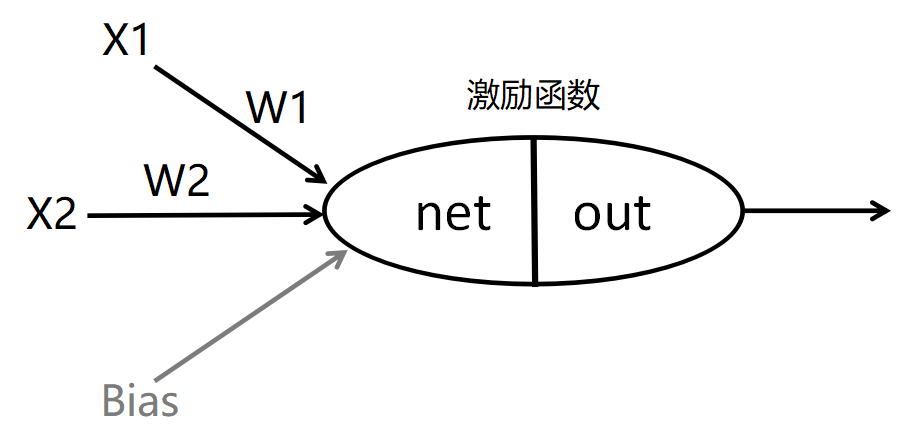
\includegraphics[width=10cm]{perceptron.png}
      \caption{感知机神经元结构}
      \label{fig:1}
  \end{figure}

  感知机的结构如图~\ref{fig:1}所示。其中,
  激励函数一般为非线性函数,将输入值映射到一个较小区间中,以提高
  感知机对非线性函数的拟合能力。
  激励函数有很多,如$Sigmoid$、$tanh$、$ReLU$等。

  本文采用最常见的Sigmoid函数作为感知机的激励函数。Sigmoid函数及其导函数可表示为:
  \begin{equation}
    Sigmoid(x)=\frac{1}{1+e^{-x}}
  \end{equation}

  \begin{equation}
    Sigmoid'(x)=Sigmoid(x)(1-Sigmoid(x))
  \end{equation}
  
  \section{多层感知机网络}

  单个感知机已被证明不能解决线性不可分问题(如异或问题),
  但多层感知机网络可以解决大多数此类问题。
  本文采用由两层感知机神经元组成的多层感知机网络,
  该网络包含输入层、隐含层与输出层。

  \begin{figure}[ht]
    \centering
      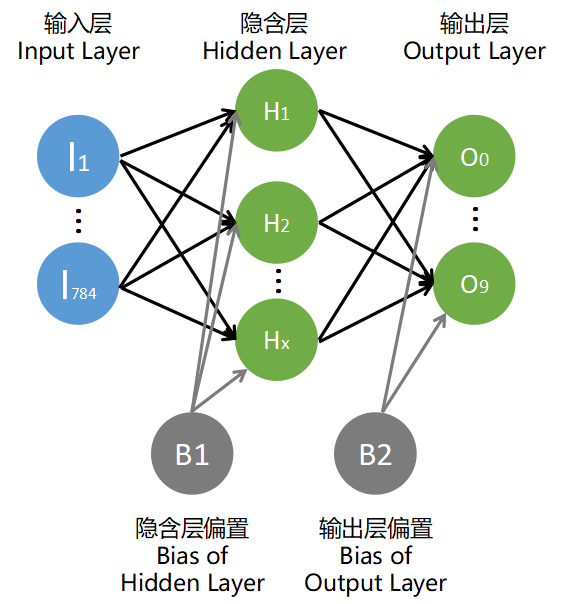
\includegraphics[width=10cm]{mlp.png}
      \caption{多层感知机网络结构}
      \label{fig:2}
  \end{figure}

  该网络结构如图\ref{fig:2}所示。其中输入层由784个结点构成,
  分别代表经归一化处理后的输入数据的每个像素点的灰度值,
  隐含层由$n_h$个感知机神经元组成,输出层由10个感知机神经元组成,
  它们的输出分别代表输入图片为数字0到9的概率。

  \section{正向传播算法}
    
    \subsection{输入数据的预处理}
    
      为了提高训练的收敛速率、最终的分类准确率,
      需要对输入数据进行归一化(Normalization)处理,
      使得输入数据由较大的区间$[0,255]$映射到区间$[0,1]$上。
      本文采用minmax归一化方法。

      设输入数据的784维中灰度值最小值为$min$,最大值为$max$,
      则该数据的第$i$维灰度值归一化为:

      \begin{equation}
        input_{i}\gets \frac{input_{i}-min}{max-min}
      \end{equation}

    \subsection{输入数据的正向传播}

      输入数据通过隐含层、输出层正向传播后得到输出结果。

      对于第$i$个隐含层神经元$h_i$,
      它接受来自输入层的784个输入值$input_j$,
      对它们加权求和并加上偏置$b_h$得到$net_{h_i}$:

      \begin{equation}
        net_{h_i}=\sum_{j=1}^{784}{w_jinput_j}+b_h
      \end{equation}

      然后经激励函数处理后得到隐含层神经元的输出值$out_{h_i}$:

      \begin{equation}
        out_{h_i}=\sigma(net_{h_i})
      \end{equation}

      对于第$i$个输出层神经元$h_i$,
      它接受来自隐含层的$n_h$个输入值$out_{h_j}$,
      对它们加权求和并加上偏置$b_o$得到$net_{o_i}$:

      \begin{equation}
        net_{o_i}=\sum_{j=1}^{n_h}{w_jout_{h_j}}+b_h
      \end{equation}

      然后经激励函数处理后得到输出层神经元的输出值$out_{o_i}$:

      \begin{equation}
        out_{o_i}=\sigma(net_{o_i})
      \end{equation}

    \subsection{误差估计}
    
    在训练过程中,输入数据经正向传播得到输出数据后,需要通过误差估计,将其与期望得到的输出数据作比对。

    误差估计的方法有很多,
    常见的有均方误差(Mean Squared Error,MSE)、交叉熵误差(Cross Entropy Error,CEE)。
    本文采用MSE作为误差估计方法。

    对于输出层的第$i$个神经元,其输出$out_{o_i}$与期望输出$output_i$之间的MSE为:

    \begin{equation}
      E_i=\frac{1}{2} (out_{o_i}-output_i)^2
    \end{equation}

    则总的MSE可表示为:

    \begin{equation}
      E=\sum_{i=0}^{9}{E_i}
    \end{equation}

  \section{反向传播算法}

    多层感知机网络中包含很多边权与偏置权重,因此需要高效的算法来调整这些权重,
    使得网络的MSE尽可能小,这一过程称之为训练(Train)。

    训练算法有很多,如反向传播算法(Error Backpropagation Algorithm,BP)、
    神经进化算法(Neuro Evolution)等,本文采用最经典的反向传播算法。

    \begin{figure}[ht]
      \centering
        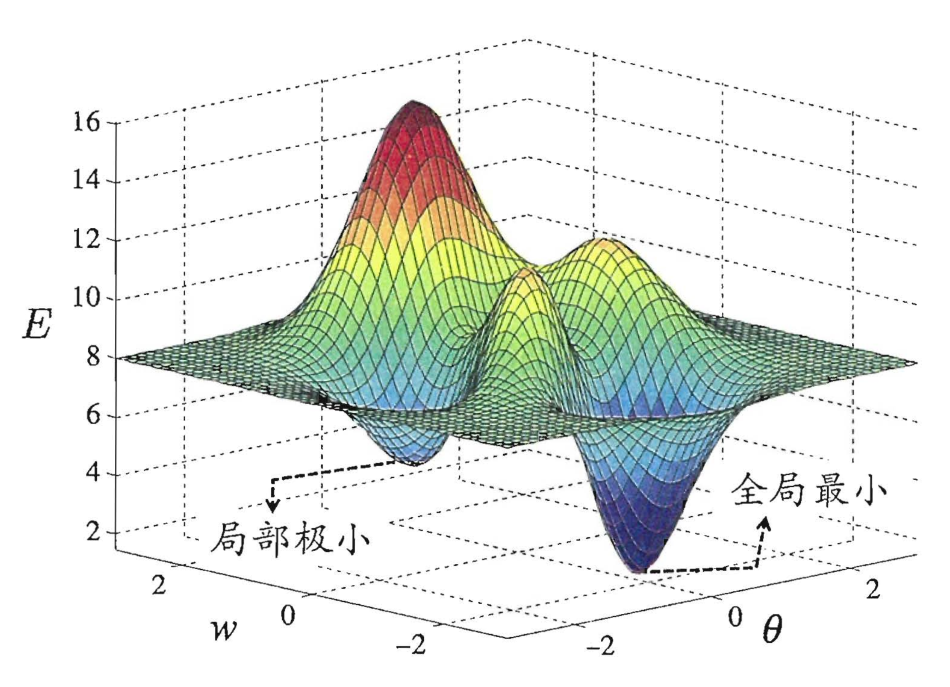
\includegraphics[width=10cm]{errorspace.png}
        \caption{全局最小与局部最小}
        \label{fig:3}
    \end{figure}

    BP算法的本质是对于每个权重,求出总MSE对该权重的偏导数,并根据偏导数
    将该权重沿使MSE减小的方向调整。

    两层结构的多层感知机网络的BP算法具体如下\upcite{zzhml}。

    \subsection{隐含层到输出层边权的权值更新}
      
      设隐含层神经元$h_i$到输出层神经元$o_j$的边权为$w_{i,j}$,则总的MSE对其的偏导数为:

      \begin{equation}
        \frac{\partial{E}}{\partial{w_{i,j}}}=
        \frac{\partial{E}}{\partial{out_{o_j}}}
        \frac{\partial{out_{o_j}}}{\partial{net_{o_j}}}
        \frac{\partial{net_{o_j}}}{\partial{w_{i,j}}}
        \label{equa11}
      \end{equation}

      其中,

      \begin{equation}
        \frac{\partial{E}}{\partial{out_{o_j}}}
        =out_{o_j}-output_j
        \label{equa12}
      \end{equation}

      \begin{equation}
        \frac{\partial{out_{o_j}}}{\partial{net_{o_j}}}
        =\sigma'(net_{o_j})
        =out_{o_j}(1-out_{o_j})
        \label{equa13}
      \end{equation}

      \begin{equation}
        \frac{\partial{net_{o_j}}}{\partial{w_{i,j}}}
        =out_{h_i}
        \label{equa14}
      \end{equation}

      将式\ref{equa12}、\ref{equa13}、\ref{equa14}代入式\ref{equa11}:
      
      \begin{equation}
        \frac{\partial{E}}{\partial{w_{i,j}}}=
        (out_{o_j}-output_j)out_{o_j}(1-out_{o_j})out_{h_i}
      \end{equation}

      定义隐含层到输出层边权的学习率为$\eta_{h,o}$,则$w_{i,j}$的更新公式为:

      \begin{equation}
        w_{i,j}\gets w_{i,j}-\eta_{h,o}\frac{\partial{E}}{\partial{w_{i,j}}}
      \end{equation}
    
    \subsection{输出层偏置的权值更新}
      设输出层偏置为$b_o$,则总的MSE对其的偏导数为:

      \begin{equation}
        \frac{\partial{E}}{\partial{b_o}}=
        \frac{\partial{E}}{\partial{out_{o_j}}}
        \frac{\partial{out_{o_j}}}{\partial{net_{o_j}}}
        \frac{\partial{net_{o_j}}}{\partial{b_o}}
        \label{equa21}
      \end{equation}

      其中,

      \begin{equation}
        \frac{\partial{E}}{\partial{b_o}}=1
        \label{equa22}
      \end{equation}

      将式\ref{equa12}、\ref{equa13}、\ref{equa22}代入式\ref{equa21}:
      
      \begin{equation}
        \frac{\partial{E}}{\partial{b_o}}=
        (out_{o_j}-output_j)out_{o_j}(1-out_{o_j})
      \end{equation}

      定义输出层偏置权值的学习率为$\eta_{b_o}$,则$b_o$的更新公式为:

      \begin{equation}
        b_o\gets b_o-\eta_{b_o}\frac{\partial{E}}{\partial{b_o}}
      \end{equation}

    \subsection{输入层到隐含层边权的权值更新}

      设输入层神经元$i_i$到隐含层神经元$h_j$的边权为$w_{i,j}$,则总的MSE对其的偏导数为:

      \begin{equation}
        \frac{\partial E}{\partial w_{i,j}}=
        \frac{\partial E}{\partial out_{h_j}}
        \frac{\partial out_{h_j}}{net_{h_j}}
        \frac{net_{h_j}}{w_{i,j}}
        \label{equa31}
      \end{equation}

      其中,
      
      \begin{equation}
        \begin{split}
        \frac{\partial E}{\partial out_{h_j}}&=
        \sum_{k=0}^9 \frac{\partial E}{\partial out_{o_k}}
        \frac{\partial out_{o_k}}{\partial net_{o_k}}
        \frac{\partial net_{o_k}}{\partial out_{h_j}} 
        \\
        &=
        \sum_{k=0}^9
        (out_{o_k}-output_k)
        out_{o_k}(1-out_{o_k})
        w_{h_j,o_k}
        \end{split}
        \label{equa32}
      \end{equation}

      \begin{equation}
        \frac{\partial out_{h_j}}{net_{h_j}}=
        out_{h_j}(1-out_{h_j})
        \label{equa33}
      \end{equation}

      \begin{equation}
        \frac{net_{h_j}}{w_{i,j}}=
        input_i
        \label{equa34}
      \end{equation}

      定义输入层到隐含层边权权值的学习率为$\eta_{i,h}$,则$w_{i,j}$的更新公式为:

      \begin{equation}
        w_{i,j} \gets w_{i,j} - \eta_{i,h} \frac{\partial E} {\partial w_{i,j}}
      \end{equation}

%%%============================================================================================================%%%

%%%=== 参考文献 ========%%%
\cleardoublepage\phantomsection
\addcontentsline{toc}{chapter}{参考文献}
\begin{thebibliography}{00}

  \bibitem{mnistdb} Lecun Y, Cortes C. The mnist database of handwritten digits[DB/OL]. 

  \bibitem{kaggle} Digit Recognizer[EB/OL]. (2018-03-18)[3/18]. https://www.kaggle.com/c/digit-recognizer.

  \bibitem{svm} Burges C J C. A Tutorial on Support Vector Machines for Pattern Recognition[J]. Data Mining and Knowledge Discovery, 1998,2(2):121-167.

  \bibitem{capsule} Sabour S, Frosst N, Hinton G E. Dynamic Routing Between Capsules[J]. CoRR, 2017,abs/1710.09829.

  \bibitem{zzhml} 周志华. 机器学习[M]. 清华大学出版社, 2016.
\end{thebibliography}

% !Mode:: "TeX:UTF-8"
%%%%%%%%%%%%%%%%%%%%%%%%%%%%-------致谢--------%%%%%%%%%%%%%%%%%%%%%%%%%%%%%%%%

\acknowledgement
\addcontentsline{toc}{chapter}{致谢}


感谢你, 感谢他和她, 感谢大家.











 %%%致谢

%%%-------------- 附录. 不需要可以删除.-----------
\appendix

\chapter{测试}

\section{第一个测试}
测试公式编号
\begin{equation}
1+1=2.
\end{equation}

表格编号测试

\begin{table}[h]
  \centering
  \caption{测试表格}
  \begin{tabular}{*{20}c}
     \hline
     % after \\: \hline or \cline{col1-col2} \cline{col3-col4} ...
     11 & 13  & 13  & 13  & 13 \\
     12 & 14  & 13  & 13  & 13 \\
     \hline
   \end{tabular}
\end{table}


\chapter{附录测试}

测试

\chapter{附录测试}

测试

\cleardoublepage
\end{document}



